\documentclass[12pt]{article}
%	options include 12pt or 11pt or 10pt
%	classes include article, report, book, letter, thesis
\usepackage{geometry}
 \geometry{
 a4paper,
 total={210mm,297mm},
 left=20mm,
 right=20mm,
 top=20mm,
 bottom=20mm,
 }
\usepackage{graphicx}
\usepackage[utf8]{inputenc}
\usepackage[obeyspaces]{url}
\usepackage{mathtools}
\usepackage{natbib}
\usepackage{listings}

\bibliographystyle{plain}
\graphicspath{{pictures/}}

\title{Reference document: Tracking Cells and Analyzing images}
\author{AMOLF \footnote{1st version by Eduardo Olimpio}}
\date{\today}

\begin{document}
\maketitle

\section{Installation}

All the guidelines here apply to Windows 7 system, but similar procedures could be followed in other operational systems. To run the tracking software described in \cite{Amat2014}, a PC with a GPU with CUDA capabilities\footnote{More information found in \url{http://docs.nvidia.com/cuda/cuda-c-programming-guide/index.html#axzz3ejDLnsIT}} is required. If you have this, install the CUDA toolkit, available in \url{https://developer.nvidia.com/cuda-downloads}.

\subsection{Download the C program}

\begin{enumerate}
\item{Download the ZIP file in \url{http://www.janelia.org/sites/default/files/Labs/Keller%20Lab/TGMM_Supplementary_Software_1_0.zip}}
\item{Unzip the file into a desired folder}
\item{Copy the file \path{$C_FOLDER$/data/TGMM_configFile.txt} to any folder you want, so that you can edit it while keeping the original\footnote{We refer to \path{$C_FOLDER$} as the folder where you extracted the C software}}
\item{It is highly recommended that you read the \path{$C_FOLDER$/README.txt} file}
\end{enumerate}

\subsection{Download GitHub}

If you do not have GitHub installed, download it from \url{https://windows.github.com/}. Be familiar with the simple git functions, it is indeed very simple and useful. The task here is to clone a repository (where the analysis code is) to your machine, in a folder that we will refer as \path{$GIT_FOLDER$}. Is you want to do it as fast as possible, follow the simple instructions (up to step 3) in \url{https://help.github.com/articles/getting-started-with-github-for-windows/}. The URL of the repository is \url{https://github.com/epolimpio/image_extraction.git}.

If you want to start to change the code from this version, just fork the project to your Desktop. This option is the best if you want to keep developing the code using the functionalities of GitHub. The instructions to do it are found in \url{https://guides.github.com/activities/forking/}.

\subsection{Install Python}

All the analysis are done in Python, so if you do not have Python installed, it is time to do so. For Windows I recommend the Anaconda distribution, but feel free to install any distribution you want. We will need some extra packages, which I explain below. The easiest way install the packages is by using the command line\footnote{Accessible in Windows by running \path{cmd.exe} in the run prompt (Windows+R in the keyboard)} and type the command:

\begin{verbatim}
conda install <package_name>
\end{verbatim}

If the package is not available, the easiest way to get it is going to \url{https://binstar.org/} and search for the package in the top left of the page. In the example below we show how to do it to install the \textit{tifffile} package.

\begin{figure}[h]
\centering
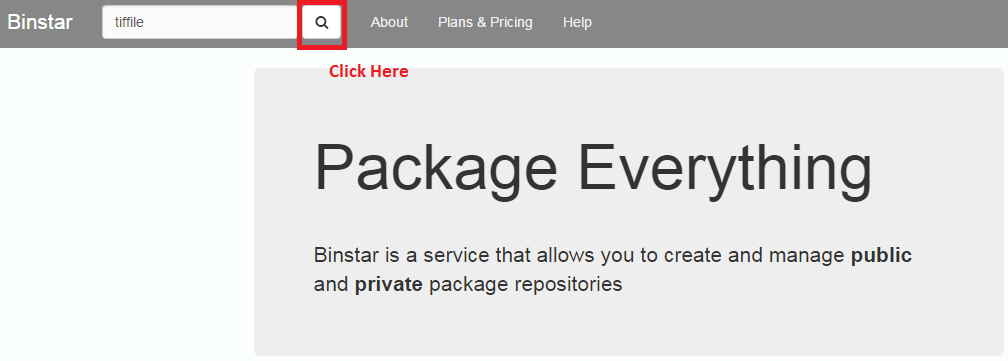
\includegraphics[width=0.8\textwidth]{binstar_search.png}
\end{figure}

\begin{figure}[h]
\centering
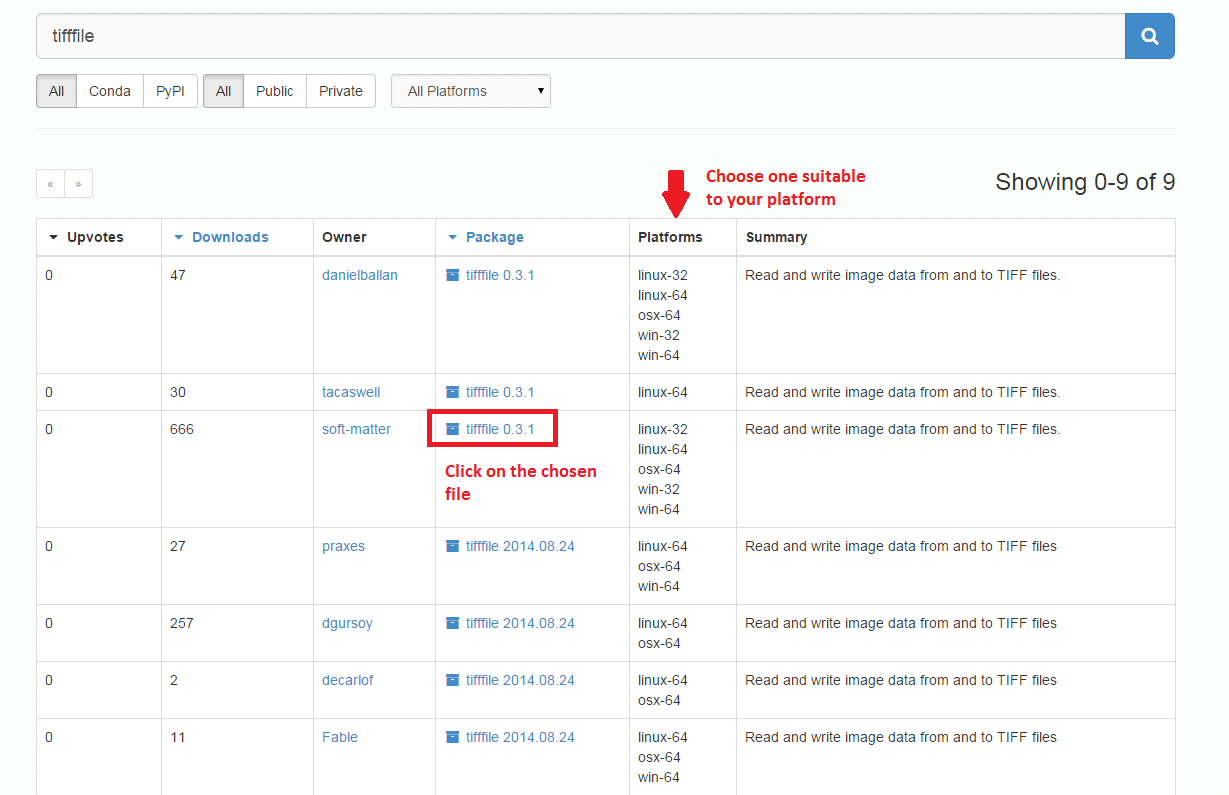
\includegraphics[width=0.8\textwidth]{binstar_package.png}
\end{figure}

\begin{figure}[h]
\centering
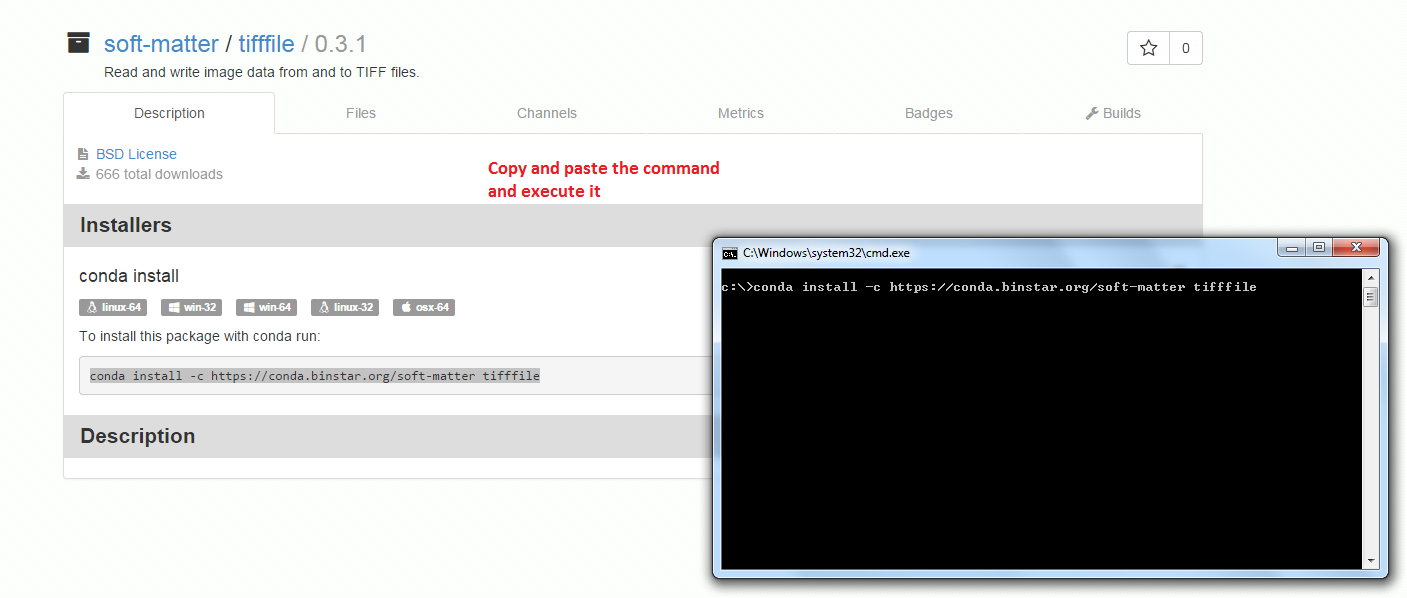
\includegraphics[width=0.8\textwidth]{binstar_install.png}
\end{figure}

\textbf{IMPORTANT NOTE:} All the development was made in Python 3 and there could be some problems running in Python 2. If you want to avoid these problems, you can create a Anaconda environment and run in Python 3 without affecting the Python 2 installation.

\subsubsection{Necessary Packages}

There are several extra packages needed to run the analysis. The packages marked with * come with the basic Anaconda installation.

\begin{enumerate}
\item{tifffile}
\item{lxml}
\item{numpy*}
\item{matplotlib*}
\end{enumerate}

\subsection{Running a test of the C software}

To figure out if the tracking software is properly working, you need to change the configuration file and run an example (already provided with the software) and check if there are results coming out from it.

\subsubsection{Changing the configuration file}

The configuration file contains many parameters used to run the tracking software. It is important to be familiar with how to use this, as explainend in \url{https://www.janelia.org/sites/default/files/Labs/Keller%20Lab/TGMM_UserGuide.v2.pdf}. Here we will teach the basics on how to run the tracking program.

\begin{enumerate}
\item{Open the copy of the configuration file you made during installation of the tracking software, in the path that we call \path{$CONFIG_PATH$}}
\item{Change the line containing imgFilePattern to imgFilePattern=\path{$C_FOLDER$/data/data/TM?????_timeFused_blending/SPC0_CM0_CM1_CHN00_CHN01.fusedStack_?????}}
\item{Change the line containing debugPathPrefix to debugPathPrefix=\path{$RESULTS_FOLDER$}}
\end{enumerate}

Here, replace \path{$C_FOLDER$} by the folder where you extracted the tracking program and \path{$RESULTS_FOLDER$} by a folder of your choice created to handle the results of the tracking program. Each run of the program will generate a new folder inside the chosen one. Remember that the folder of the variable imgFilePattern MUST use slash and for debugPathPrefix you MUST use backslash.

\subsubsection{Changing the batch file}

The batch files are used to make it easier to run the tracking software. There are three different batch files in the folder \path{$GIT_FOLDER$}:

\begin{enumerate}
\item{\path{segmentation.bat}: Used to run the pre-Track program, required to run the main program.}
\item{\path{bayesian_pos.bat}: Runs the main program}
\item{\path{seg_analysis.bat}: Used to run the segmentation analysis in debug (with report) if the segmentation program fails.}
\end{enumerate}

We need to change these files to provide them with the right path. To edit these files, right click on them and select ``Edit''. The changes you must provide in all of them are the same. You need to change the line with \path{c_folder} to include the path you extracted the tracking software (referred here as \path{$C_FOLDER$}) and the line containing the set of \path{config_path} should be changed to \path{$CONFIG_PATH$}.

\subsubsection{Running the software} \label{sec_run_c_tracking}

To run the program now, just execute the file \path{segmentation.bat} (double/click or use command line) and use initial frame 0 and final frame 30. If the program has sucessfully run, you will get the message \textit{``Hierarchical segmentation ran successfully''}. Then you can run the file \path{bayesian_pos.bat} and use again initial frame 0 and final frame 30. If everything runs OK, you will find a new folder inside the \path{$RESULTS_FOLDER$} in a format similar to \path{GMEMtracking3D_yyyy_mm_dd_hh_mm_ss} and inside it you will have two folders with the XML and the binary (\path{.svb}) files, and a \path{.txt} with the log of your run.

\section{Running the Tracking Software and the Analysis}

In order to analyze the data, you need to follow the steps:

\begin{enumerate}
\item{Cut the area of interest and make the data compatible to that required by the tracking software}
\item{Run the tracking algorithm}
\item{Run the eye check procedure to generate the analysis image}
\item{Curate the data using the manual track}
\end{enumerate}

\subsection{Before running the track analysis} \label{sec_run_pre_track}

Before running the analysis make sure that the TIFF images are 16-bit. The program runs only for 8-bits or 16-bits one color images. Usually the images come in different folders (one for each time step) and with several stacks per time frame (for 3D compositions). Therefore, the path pattern resembles something like \path{../T?????/T?????Z@@@} where the symbols \path{?} and \path{@} are replaced by the corresponding time and stack integers. As an example, for the second frame (Time = 2) and the tenth stack (Z = 10) we have \path{../T?????/T?????Z@@@}.

To generate the stacked TIFF image, you need to run the script \path{gen_stacks_for_tracking.py}, following the steps:

\begin{enumerate}
\item{Copy the file \path{config_stacked_images.conf} to the image folder (we will call it \path{$IM_FOLDER$}). The path of the copied configuration file is \path{$IM_CONFIG_PATH$}.}
\item{Check the images, contained in the path (example) \path{$IM_FOLDER$/T?????/T?????Z@@@} and see how you want to cut the images (if needed). To check the cutting parameters, use a nice image visualizing software. In Figure \ref{fig_cutting} we use IrfanView as an example.}
\item{Edit the configuration file (in \path{$IM_CONFIG_PATH$}) and include all the parameters required (section \ref{sec_write_cut_config})}
\item{Open the command window, go to the \path{$GIT_FOLDER$} and execute \path{py gen_stacks_for_tracking.py <$IM_CONFIG_PATH$>}}
\end{enumerate}

\subsubsection{Writing the configuration file} \label{sec_write_cut_config}

The program generates the stacked TIFF file cut in the region you chose and output it according to the pattern you choose. All the required parameters are saved in the file \path{$IM_CONFIG_PATH$}, called together with the function. An example file is below:

\begin{verbatim}
# ====================================================
# number of time frames
n_time = 129

# initial time
t_ini = 1

# number of z-components per time frame
n_z = 29

# Cutting parameters, used only if cut = True
cut = True
cut_x = 600 
cut_y = 500
pos_x = 300
pos_y = 200

# In - out file path
path_in = "D:\\data\\25 tif\\T?????C01Z@@@.tif"
path_out = "D:\\data\\25 tif\\T?????C01.tif"
# ===================================================
\end{verbatim}

\begin{enumerate}
\item{\textbf{n\_time:} Number of frames to be included in the stacked file}
\item{\textbf{t\_ini:} Starting frame number. In the present example it starts at $T=1$ and goes until $T=129$}
\item{\textbf{n\_z:} Number of stacks to be included (the first is assumed to be 1)}
\item{\textbf{cut:} True is you want to cut, False if not}
\item{\textbf{pos\_x, pos\_y:} Define the corner position of the region to be cut}
\item{\textbf{cut\_x, cut\_y:} Size of the region to be cut}
\item{\textbf{path\_in:} Input pattern, use \path{?} for the time and \path{@} for Z}
\item{\textbf{path\_out:}  Output pattern of the stacked image, use \path{?} for the time}
\end{enumerate}

To illustrate how to choose the cut parameters, we used IrfanView to select the desired region and show how to determine the parameters in Figure \ref{fig_cutting}.

\begin{figure}[h]
\centering
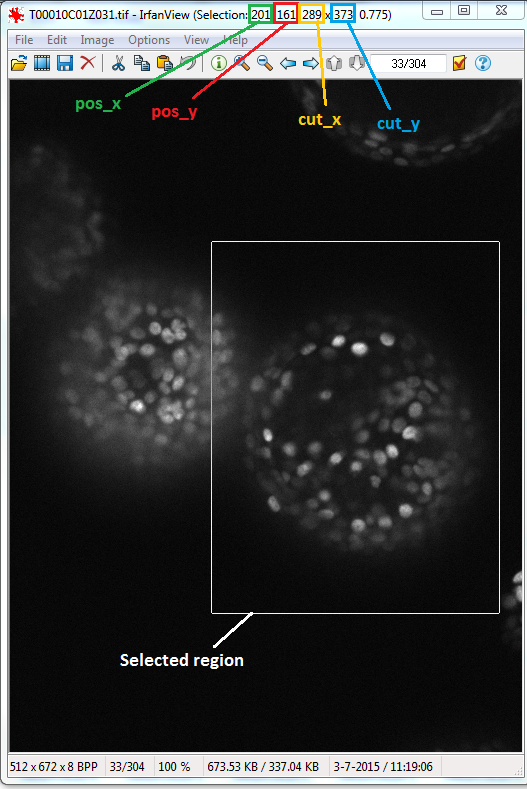
\includegraphics[width=0.6\textwidth]{cutting_region.png}
\caption{Cutting region determination \label{fig_cutting}}
\end{figure}

\bibliography{References.bib}

\end{document}